\documentclass{beamer}

\usetheme{default}
\usecolortheme{rose}
\usepackage{hyperref}
\newcommand{\ignore}[1]{}
\newcommand{\pr}{\mathbb{P}}
\newcommand{\var}{\text{var}}
\newcommand{\E}{\mathbb{E}}
\setbeamerfont{alerted text}{series=\itshape}
\addtobeamertemplate{navigation symbols}{}{%
    \usebeamerfont{footline}%
    \usebeamercolor[fg]{footline}%
    \hspace{1em}%
    \insertframenumber/\inserttotalframenumber
}

\title{Model for Counts}

% A subtitle is optional and this may be deleted
\subtitle{STAT-UB.0001 Statistics for Business Control}

\author{Ningshan Zhang}
% - Give the names in the same order as the appear in the paper.
% - Use the \inst{?} command only if the authors have different
%   affiliation.

\institute[New York University] % (optional, but mostly needed)
{
  IOMS Department\\
  nzhang@stern.nyu.edu
  \let\thefootnote\relax\footnotetext{\tiny{*  Office Hours: Wed \& Fri 10:00 - 11:30 AM, KMC 8-174}}
}
\date{Jul 17, 2018}
\AtBeginSubsection[]
{
  \begin{frame}<beamer>{Outline}
    \tableofcontents[currentsection,currentsubsection]
  \end{frame}
}

% Let's get started
\begin{document}

%-------------------
\begin{frame}
  \titlepage
\end{frame}



% Section and subsections will appear in the presentation overview
% and table of contents.
\begin{frame}{Review}
Random Variable
\begin{itemize}
\item Probability distribution function (PDF)
    \item Expected value of a random variable
    \item Variance and standard deviation of a random variable
    \item Properties of expected value
\begin{itemize}
\item Affine transformation
\item Sum
\end{itemize}
\end{itemize}
\end{frame}

\begin{frame}{Example}
A biased coin has a 25\% of landing heads, and a 75\% chance of landing tails.
If you flip the coin 4 times, what is the chance of getting exactly 2 heads?

\vspace{\stretch{0.2}}
Random variable $X$ = number of heads out of 4 flips. How to find $p(2)$?
\small
\begin{enumerate}[(a)]
\vspace{\stretch{0.4}}
\item What are the sample points that lead to the observation $X=2$?  How many are there?
\vspace{\stretch{0.4}}
\item What is the probability for each of the sample points in (a)?
\vspace{\stretch{0.4}}
\item What is $p(2)$?
\vspace{\stretch{0.4}}
\item What is $p(2)$ if you flip the coin 10 times?
\end{enumerate}
\normalsize
\end{frame}

\begin{frame}{Binomial Random Variable and Binomial Distribution}
Binomial experiment:
\begin{itemize}
\item It consists of a fixed number \alert{$n$} of statistically independent trials;
\item each trial has the same probability of success \alert{$p$};
\item we want to count the number of successes.  
\end{itemize}

\vspace{\stretch{0.2}}
Let $X$ = the number of successes. Then X is a \alert{binomial random variable} that has \alert{binomial distribution}, 
written as $X \sim B(n,p)$. The PDF:
$$
\pr(X=k) = \binom{n}{k} p^k (1-p)^{n-k}.
$$
\end{frame}

\begin{frame}{The Binomial Distribution}
If $X\sim B(n,p)$, then it has the following properties:
\begin{align*}
\pr(X=k) &= \binom{n}{k} p^k (1-p)^{n-k}, \tag{PDF}\\
\E(X) & = np, \tag{mean} \\
\var(X) &= np(1-p).\tag{variance}
\end{align*}
\end{frame}

\begin{frame}{The Binomial Distribution}
Characteristics of a Binomial Experiment:
\begin{itemize}
\item The experiment consists of $n$ identical and independent trials.
\item There are only two possible outcomes (success and failure) on each trial.
\item The probability of success is the same on each trial.
\item The random variable of interest is the number of successes out of $n$ trials.
\end{itemize}
\end{frame}


\begin{frame}{Example}
\small
The manager at NYU bookstore wants to figure out how many customers will visit the store between 4 - 5 pm.
By examining past records, he finds that on average 20.3 customers will visit the store within that hour.
%What is the probability of having 10 people visit the store? What about 20 people? 30 people? etc.
Let X = number of customers visit the store between 4 - 5 pm. What is the PDF of X? 
\vspace{\stretch{0.1}}
\begin{itemize}
\small
\item Approximate $X$ with the outcome of 60 independent trials: whether a customer visits the store in a given minute. 
\item Approximate $X$ with the outcome of 3600 independent trials:  whether $\cdots$ in a given second. 
\item Getting more and more granular, leads to the \alert{Possion distribution}.
\end{itemize}
\normalsize
\end{frame}


\begin{frame}{The Poisson Distribution}
Let $X$ = the number of events that occur in a fixed interval of time, space, etc.  Assume that
\begin{itemize}
\item Events occur with a known constant rate.
\item The events occur independently of the time since the last event.
\end{itemize}

\vspace{\stretch{0.1}}
Then $X$ follows a \alert{Poisson distribution}.
\end{frame}

\begin{frame}{The Poisson Distribution}
The PDF of Poisson distribution
$$
\pr(X=k)=\frac{\lambda^k e^{-\lambda}}{k!},
$$
\begin{itemize}
\item $k=0,1,2,\dots$. There is no upper limit on $k$ (unlike binomial).
\item $\lambda$ is the (only) parameter of the distribution.
\item $e\approx 2.72$ is a constant, the base of the natural logarithm.
\end{itemize}

\vspace{\stretch{0.1}}
Mean and variance of $X$: 
$$ \E(X)=\var(X)=\lambda.$$
\end{frame}

\begin{frame}{The Poisson Distribution: Example}
\small
The manager at NYU bookstore wants to figure out how many customers will visit the store between 4 - 5 pm.
By examining past records, he finds that on average 20.3 customers will visit the store within that hour.
Let X = number of customers visit the store between 4 - 5 pm. What is the PDF of X? 

\vspace{\stretch{0.2}}
Solution: $X$ follows a Poisson distribution with $\lambda=20.3$. Then,
\begin{itemize}
\item What is the probability of $X=10$?
$$\pr(X=10)=\frac{\lambda^{10} e^{-\lambda}}{10!}$$
\item What is the probability of $X=20$?
$$\pr(X=20)=\frac{\lambda^{20} e^{-\lambda}}{20!}$$
\end{itemize}
\end{frame}

\begin{frame}{Connection between Binomial and Poisson Distribution}
In binomial distribution, let $n\to \infty$, $p\to 0$, but keep the mean as a constant: $np=\lambda$.
Then,
$$ B(n,p) \to \text{Poisson}(\lambda).$$

Proof: for any fixed number $k$ and parameter $\lambda$,
\small
\begin{align*}
& \binom{n}{k} p^k (1-p)^{n-k} \tag{PDF of $X\sim B(n,p)$}\\
&= \frac{n!}{k! (n-k)!} \left(\frac{\lambda}{n}\right)^k \left(1-\frac{\lambda}{n}\right)^{n-k}  \\
    &= \frac{\lambda^k}{k!} \underbrace{\left[\frac{n(n-1)\cdots (n-k+1)}{n^k}\right]}_{\to 1}
    \underbrace{\left(1-\frac{\lambda}{n}\right)^{n}}_{\to e^{-\lambda}}
    \underbrace{\left(1-\frac{\lambda}{n}\right)^{-k}}_{\to 1}\\
    & \to \frac{\lambda^k e^{-\lambda}}{k!}   \tag{PDF of $X \sim \text{Poisson}(\lambda)$}
\end{align*}
\end{frame}

\begin{frame}{Empirical Rule}
Empirical rule works for binomial distribution and Poisson distribution.
\begin{itemize}
\item $X\sim B(n,p)$, then $\mu=np$, $\sigma=\sqrt{np(1-p)}$.
\item $X\sim \text{Poisson}(\lambda)$, then $\mu=\lambda$, $\sigma=\sqrt{\lambda}$.
\end{itemize}
\end{frame}

\begin{frame}{Summary}
\begin{itemize}
\item Binomial random variable and binomial distribution.
\item Poisson random variable and Poisson distribution.
\item Empirical rule applies to both.
\end{itemize}

\end{frame}
\ignore{
%-------------------
\begin{frame}{Time Series Plot}
\begin{figure}
    \caption{}
    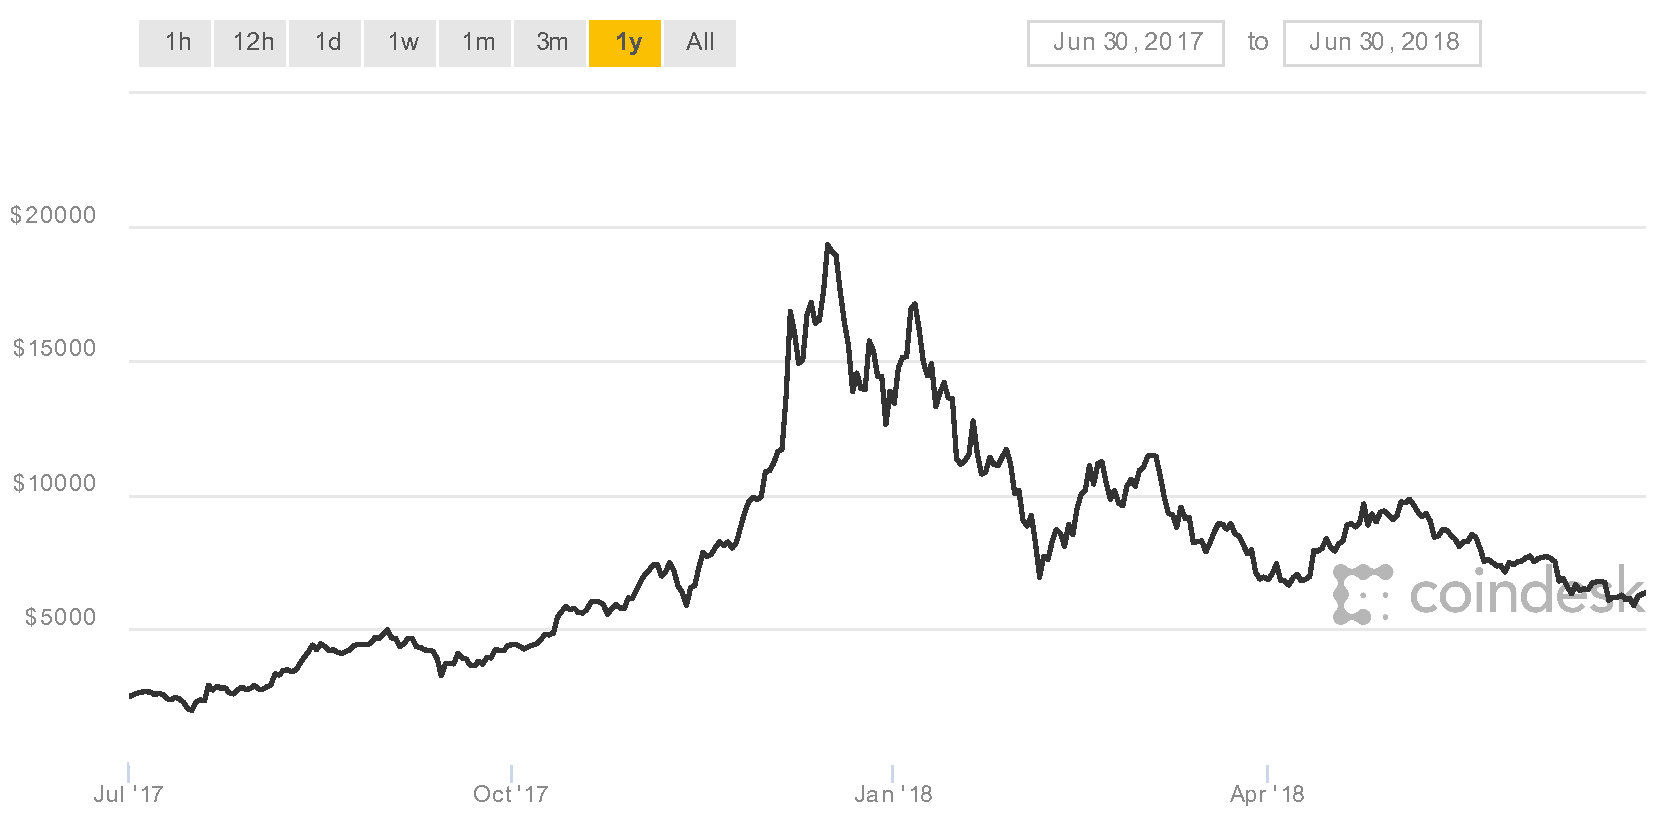
\includegraphics[width=1\textwidth]{figures/coindesk-bpi-chart}
\end{figure}
\let\thefootnote\relax\footnotetext{\tiny{* Plot from Coindesk.com}}
\end{frame}

\begin{frame}{}
\begin{itemize}
\item 
\end{itemize}
\end{frame}

\vspace{\stretch{0.5}}

\begin{block}{}
\end{block}


}

\end{document}


